\subsection{Mantle melting curves}\label{sec:katz}
This instantaneous experiment is performed in order to recreate isobaric melting curves, as function of temperature, bulk water and content of water in the
melt, to compare with melting curves obtained by \citet{Katz2003}. The domain is square with $L_x=L_y=100$ km, a grid resolution of $100\times100$ elements and
25 markers per element. Density is set in the entire domain to \SI{3300}{\kg\per\cubic\m} and temperature increases from the sides to the centre from 1000° to
1500°C. The experiment is performed for bulk water contents from 0 to 0.3 wt.\%.

Fig. \ref{fig:fraction} shows isobaric melting curves for \SI{1}{\giga\pascal} (panel a) and \SI{3}{\giga\pascal} (panel b) calculated for different bulk water
contents. The curves well match with those obtained for the mantle by \citet{Katz2003}, showing the saturation at the solidus for bulk water of 0.2 and 0.3 wt.\%, indicating
that the code correctly determines melt fraction as function of pressure, temperature and bulk water content. Same results can be observed in Fig.
\ref{fig:water}a, where isobaric and isothermal melting curves are shown as function of bulk water content. In addition, Fig. \ref{fig:water}b shows that the
code correctly determines also the percentage of water in the melt as function of pressure, temperature and melt fraction. 
All data can be found at \url{https://github.com/aleregorda/Benchmarks/tree/main/Melting}.

\begin{figure}[h!]
\centering
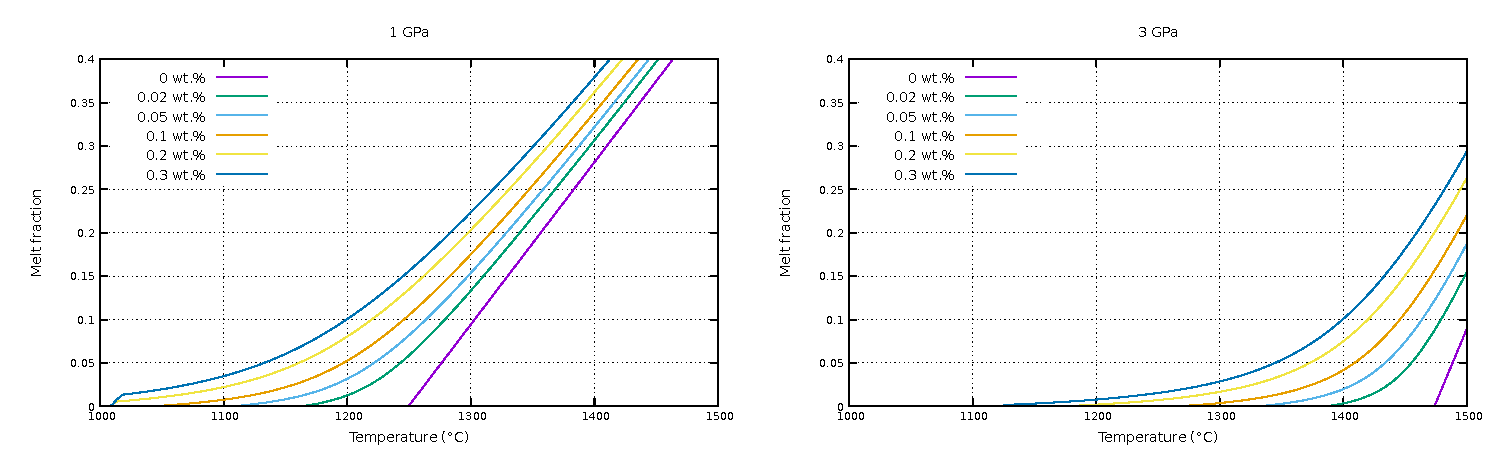
\includegraphics[width=16cm]{./Figures/Fraction.pdf}
\caption{Isobaric melting curves for 1 GPa (panel a) and 3 GPa (panel b) as function of temperature with different bulk water contents.}
\label{fig:fraction}
\end{figure}

\begin{figure}[h!]
\centering
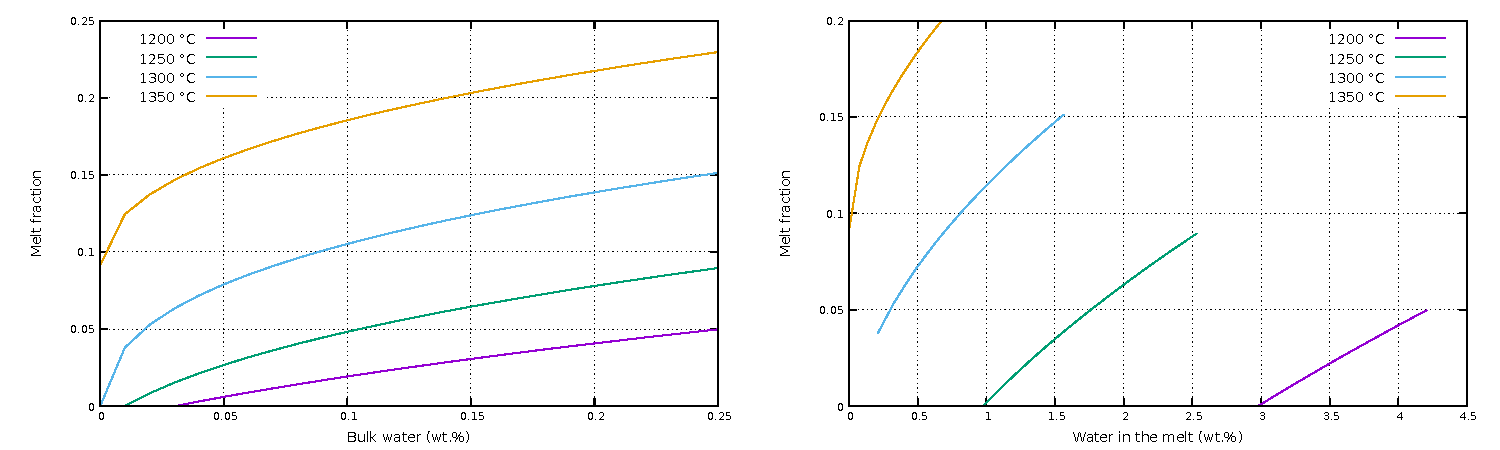
\includegraphics[width=16cm]{./Figures/Water.pdf}
\caption{Isobaric melting curves for 1.5 GPa as function of bulk water (panel a) and water in the melt (panel b) calculated for different temperatures.}
\label{fig:water}
\end{figure}